\chapter{Utilizzo della piattaforma}

Dopo la prima installazione la piattaforma si presenta, come mostrato in figura \ref{fig:demo-1-ckan-vergine}, con un�interfaccia sobria e  pronta a contenere i dataset che varranno caricati.

\begin{figure}[htbp]
   \centering
   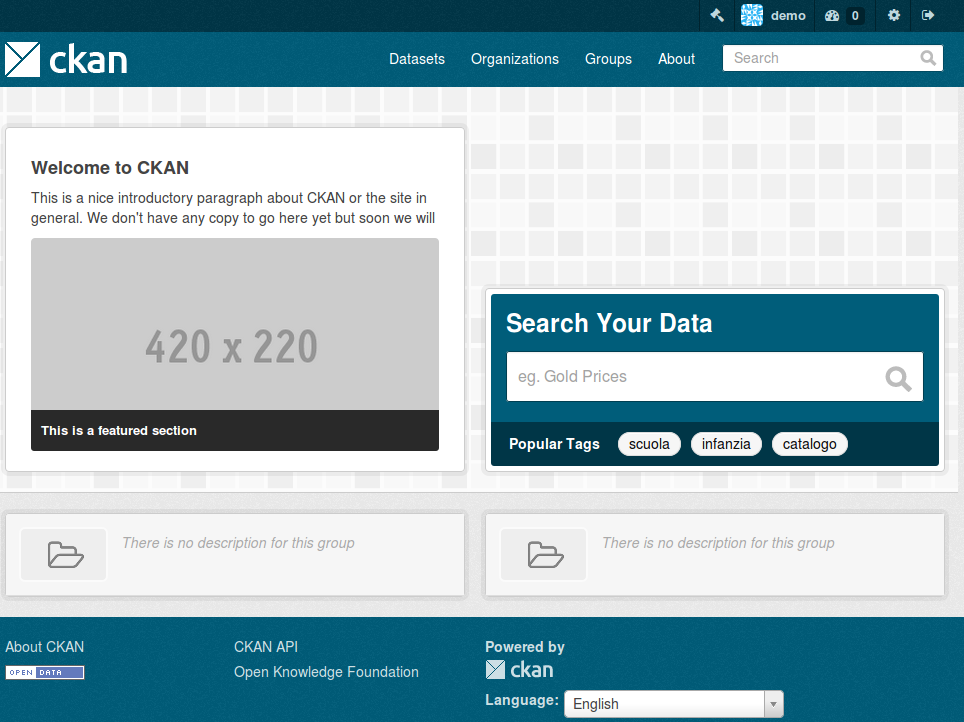
\includegraphics[scale=0.42]{img/demo-1-ckan-vergine}
   \caption{Aspetto di CKAN appena installato}
   \label{fig:demo-1-ckan-vergine}
\end{figure}

\newpage
Navigando alla voce di men� �Dataset� � possibile vedere l�elenco dei dataset disponibili, ma anche crearne uno nuovo attraverso il pulsante presente in alto a destra (figura \ref{fig:demo-2-ckan-creazione-dataset}).

\begin{figure}[htbp]
   \centering
   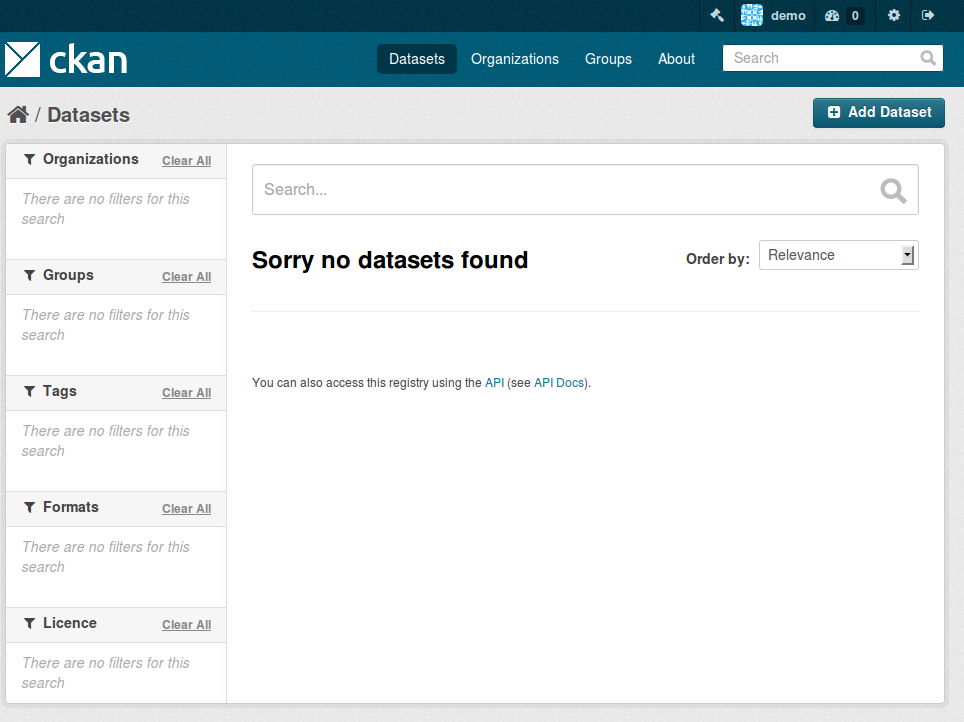
\includegraphics[scale=0.42]{img/demo-2-ckan-creazione-dataset}
   \caption{Elenco dei Dataset vuoto}
   \label{fig:demo-2-ckan-creazione-dataset}
\end{figure}

\newpage
L�inserimento di un nuovo Dataset inizia con la richiesta di inserimento delle meta-informazioni necessarie alla sua identificazione (figura \ref{fig:demo-3-ckan-primo-passo}), ovvero il titolo e la descrizione; l�utente pu� anche decidere di inserire opzionalmente alcuni tag per facilitarne la ricerca e la licenza da un elenco predefinito.

\begin{figure}[htbp]
   \centering
   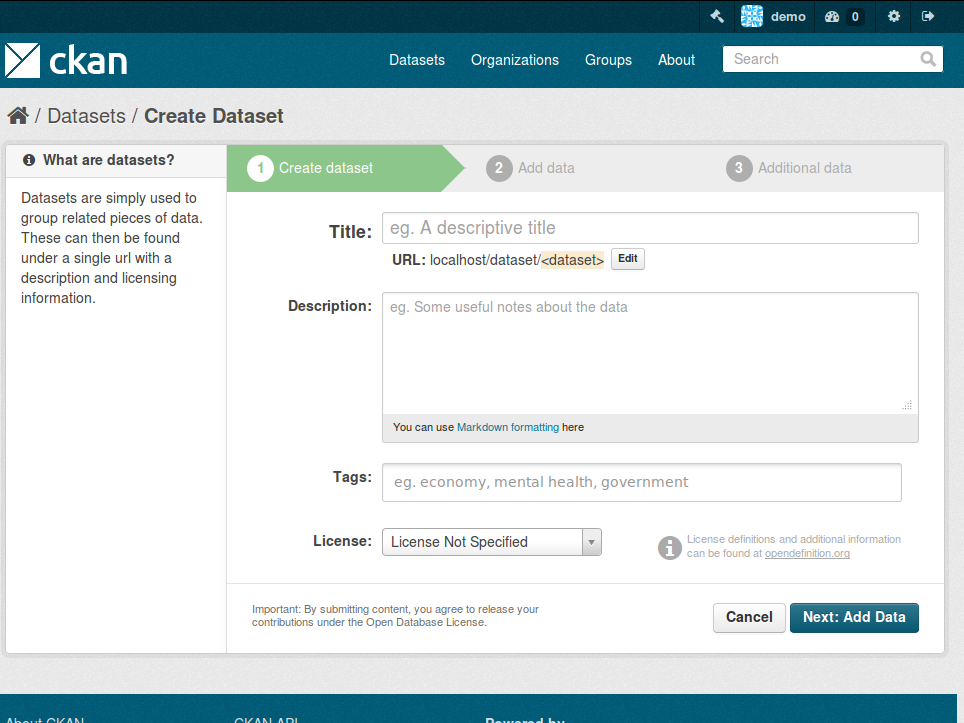
\includegraphics[scale=0.42]{img/demo-3-ckan-primo-passo}
   \caption{Definizione dei metadati durante la creazione di un dataset}
   \label{fig:demo-3-ckan-primo-passo}
\end{figure}

\newpage
Ad esempio possiamo inseriti i metadati necessari alla creazione del catalogo (figura \ref{fig:demo-3-ckan-primo-passo-condati}) per poi passare all�aggiunta dei dati veri e prorpi.

\begin{figure}[htbp]
   \centering
   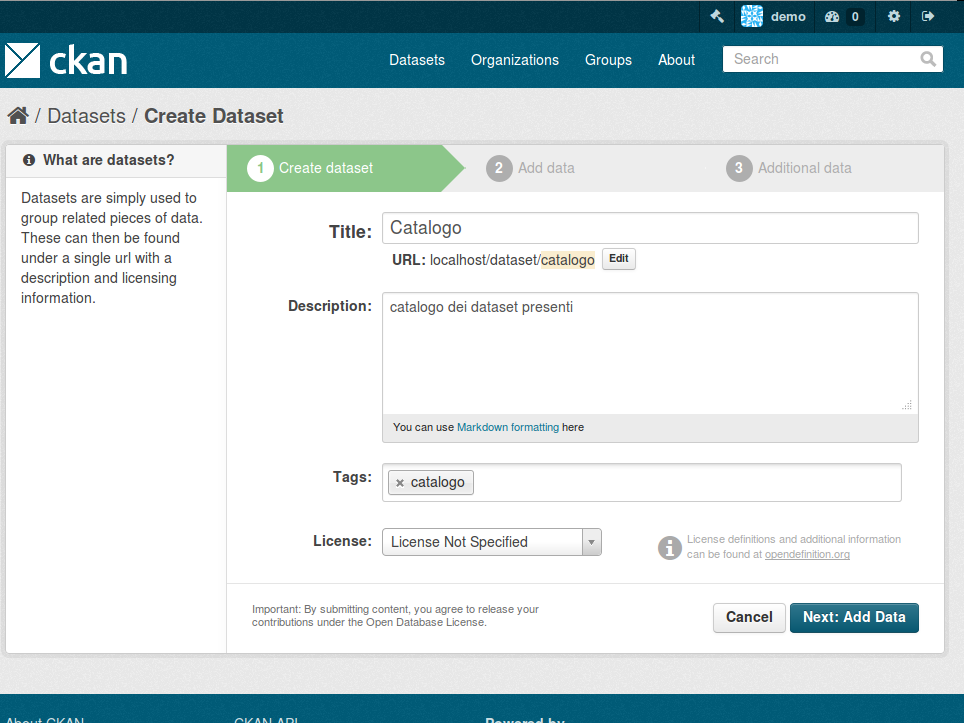
\includegraphics[scale=0.42]{img/demo-3-ckan-primo-passo-condati}
   \caption{Inserimento metadati del catalogo}
   \label{fig:demo-3-ckan-primo-passo-condati}
\end{figure}

\newpage
Nel secondo passaggio � possibile linkare un file o una risorsa esterna e specificare il nome e la descrizione che verranno utilizzati nella piattaforma (figura \ref{fig:demo-4-ckan-secondo-passo-condati}). Il formato del file viene identificato automaticamente, in caso ci� non avvenga � possibile inserirlo manualmente.

\begin{figure}[htbp]
   \centering
   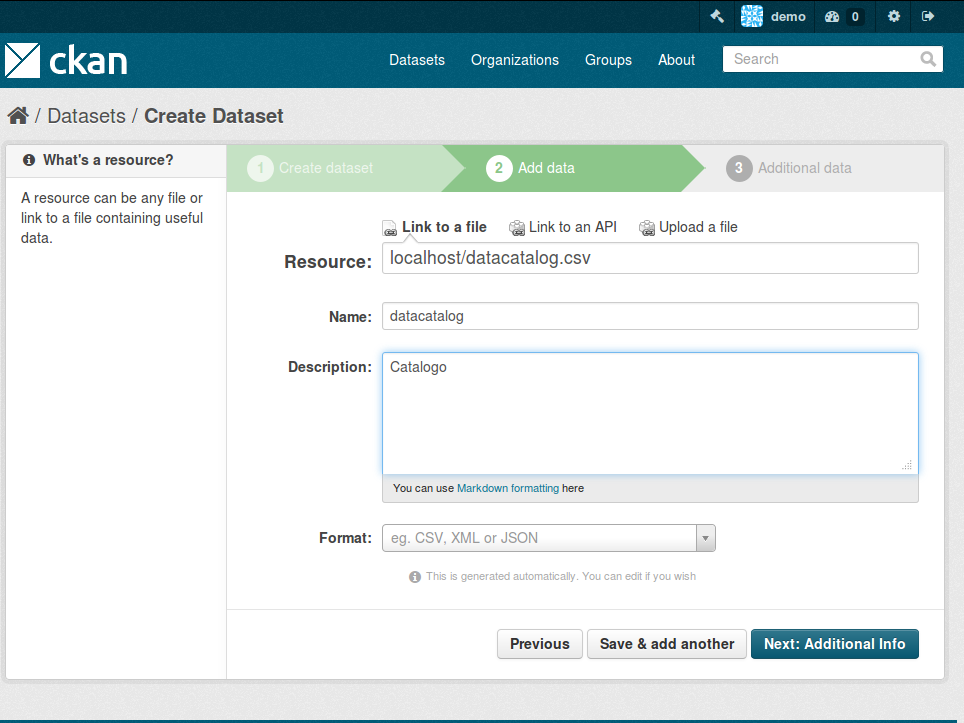
\includegraphics[scale=0.42]{img/demo-4-ckan-secondo-passo-condati}
   \caption{Inserimento risorsa nel dataset}
   \label{fig:demo-4-ckan-secondo-passo-condati}
\end{figure}

\newpage
In alternativa, una volta attivato il File Store � possibile caricare un file dal proprio computer in modo che venga memorizzato nel server (figura \ref{fig:demo-7-upload-scuola}). Un messaggio ci avvertir� del successo dell�upload o dell�eventuale fallimento nella parte alta dello schermo.

\begin{figure}[htbp]
   \centering
   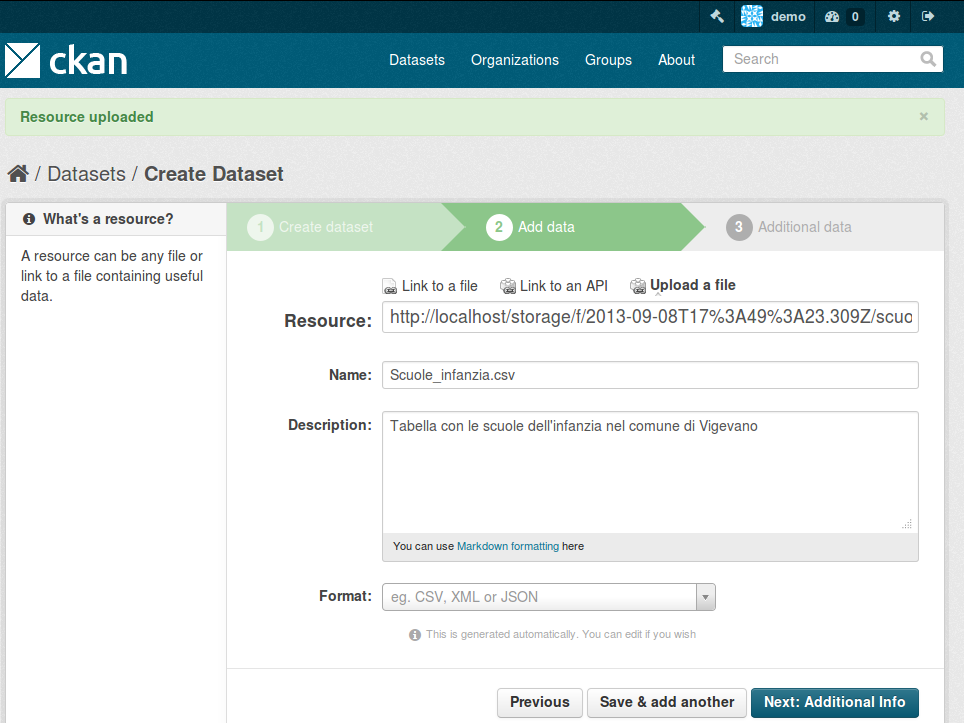
\includegraphics[scale=0.42]{img/demo-7-upload-scuola}
   \caption{Upload fine in CKAN}
   \label{fig:demo-7-upload-scuola}
\end{figure}

\newpage
Infine � possibile aggiungere ulteriori informazioni riguardanti l�autore dei dati e il manutentore (colui che si preoccupa di aggiornare il dataset nel tempo). Inoltre � possibile assegnare in dataset ad un gruppo (figura \ref{fig:demo-5-ckan-terzo-passo-condati}).

\begin{figure}[htbp]
   \centering
   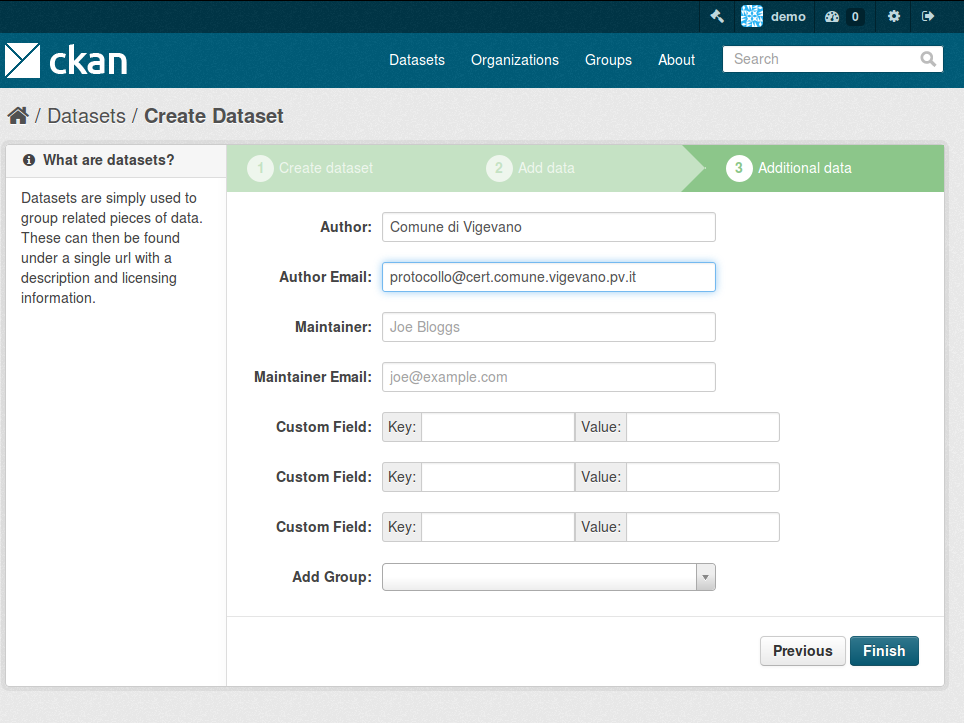
\includegraphics[scale=0.42]{img/demo-5-ckan-terzo-passo-condati}
   \caption{Inserimento dati addizionali del dataset}
   \label{fig:demo-5-ckan-terzo-passo-condati}
\end{figure}

\newpage
A questo punto ci viene mostrato il dataset con tutte le informazioni che abbiamo inserito (figura \ref{fig:demo-6-ckan-catalogo-vuoto}). Finch� il DataStorer non entra in funzione la preview non sar� disponibile.

\begin{figure}[htbp]
   \centering
   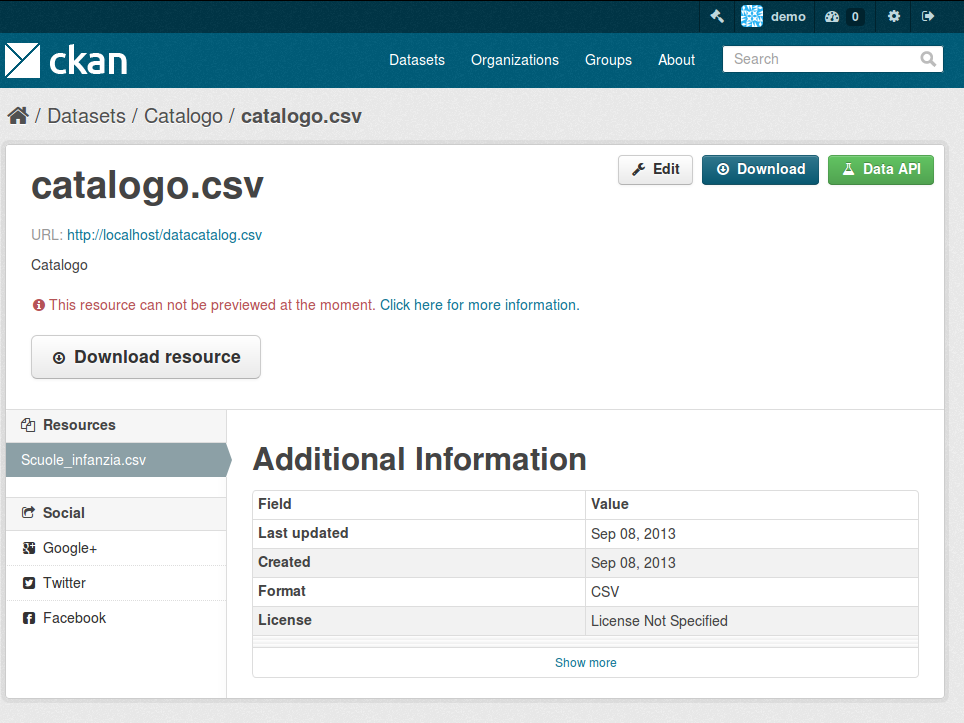
\includegraphics[scale=0.42]{img/demo-6-ckan-catalogo-vuoto}
   \caption{Dataset appena caricato, il DataStorer non � ancora entrato in funzione}
   \label{fig:demo-6-ckan-catalogo-vuoto}
\end{figure}

\newpage
Una volta che il file sar� processato e i dati contenuti nel dataset saranno salvati nel DataStore e la pagina si presenter� come mostrato in figura \ref{fig:demo-9-dataset-preview}.

\begin{figure}[htbp]
   \centering
   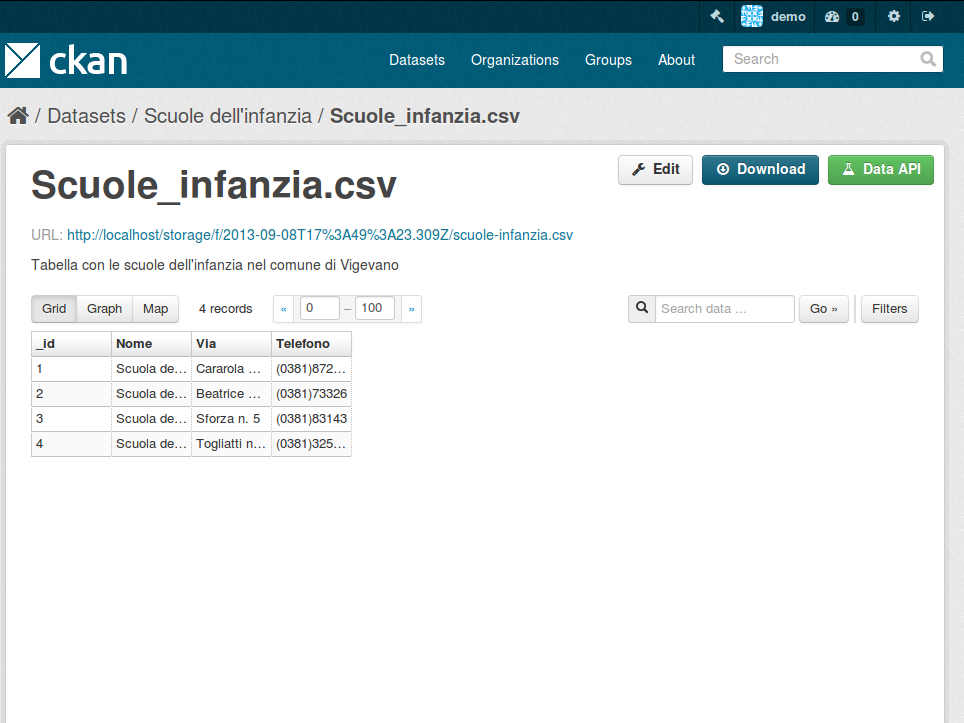
\includegraphics[scale=0.42]{img/demo-9-dataset-preview}
   \caption{Dataset con le informazioni memorizzato nel DataStore}
   \label{fig:demo-9-dataset-preview}
\end{figure}

\newpage
L�interfaccia grafica � personalizzabile rispetto alle esigenze e nel nostro caso � stata adattata per il Comune di vigevano (figura \ref{fig:demo-10-home-vigevano}).

\begin{figure}[htbp]
   \centering
   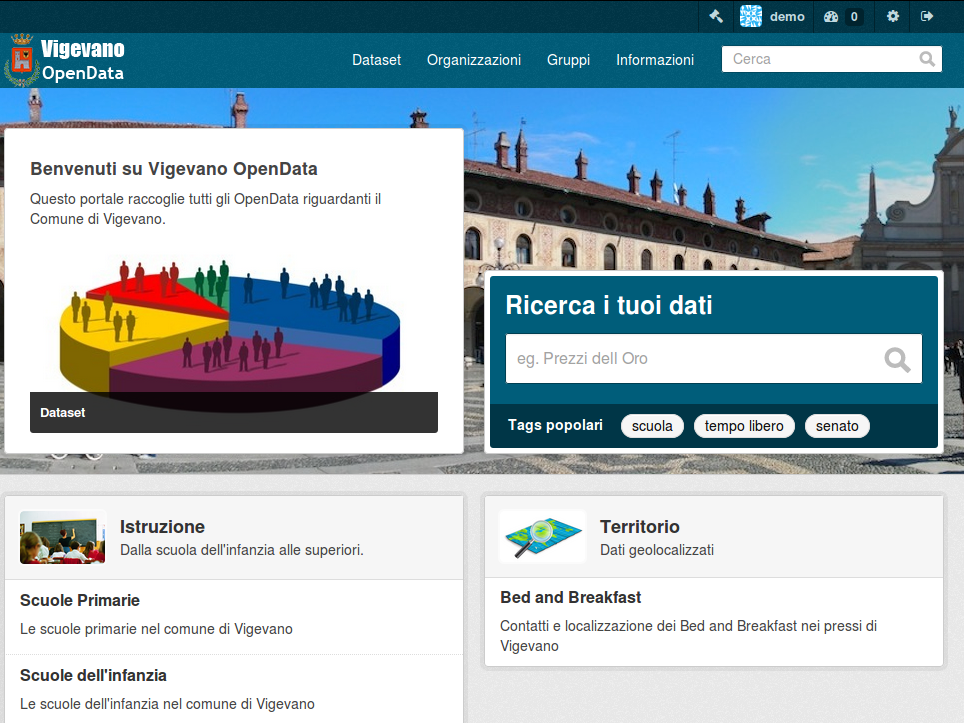
\includegraphics[scale=0.42]{img/demo-10-home-vigevano}
   \caption{Homepage di CKAN realizzato per il Comune di Vigevano}
   \label{fig:demo-10-home-vigevano}
\end{figure}

\newpage
Come mostrato in figura \ref{fig:demo-11-gruppi} � possibile suddividere i dataset per gruppi tematici, una funzione molto apprezzata dagli utenti che ricercano le informazioni di una determinata categoria.

\begin{figure}[htbp]
   \centering
   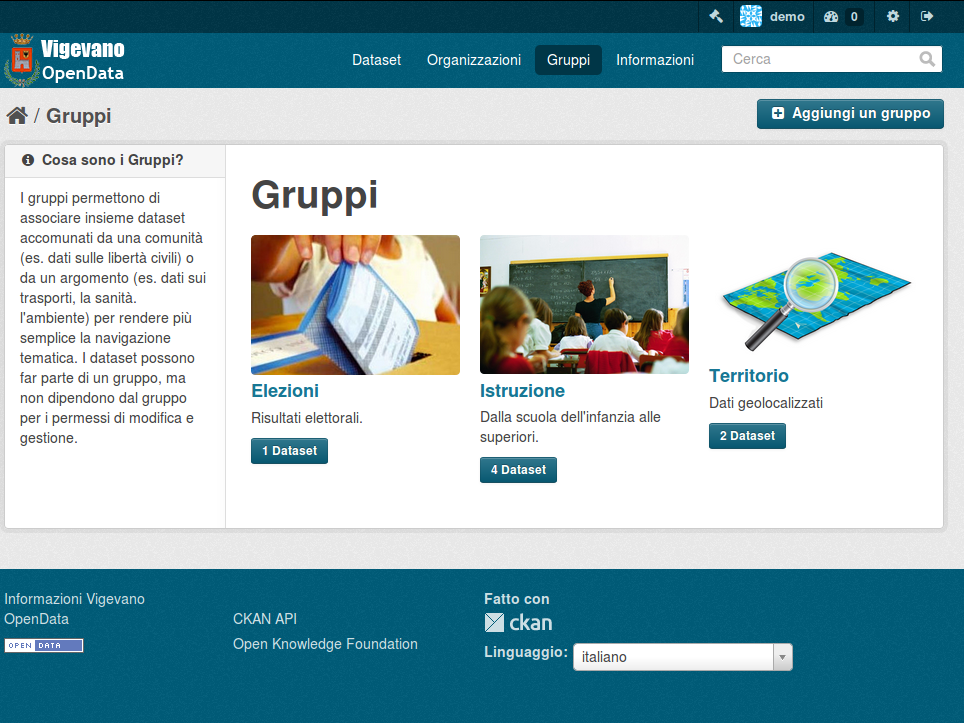
\includegraphics[scale=0.42]{img/demo-11-gruppi}
   \caption{Elenco dei gruppi di dataset disponibili}
   \label{fig:demo-11-gruppi}
\end{figure}

\newpage
Una volta entrati nella pagina di un gruppo viene presentato l�elenco dei dataset disponibili con al relativa descrizione e formato (figura \ref{fig:demo-12-gruppo-dettaglio}).

\begin{figure}[htbp]
   \centering
   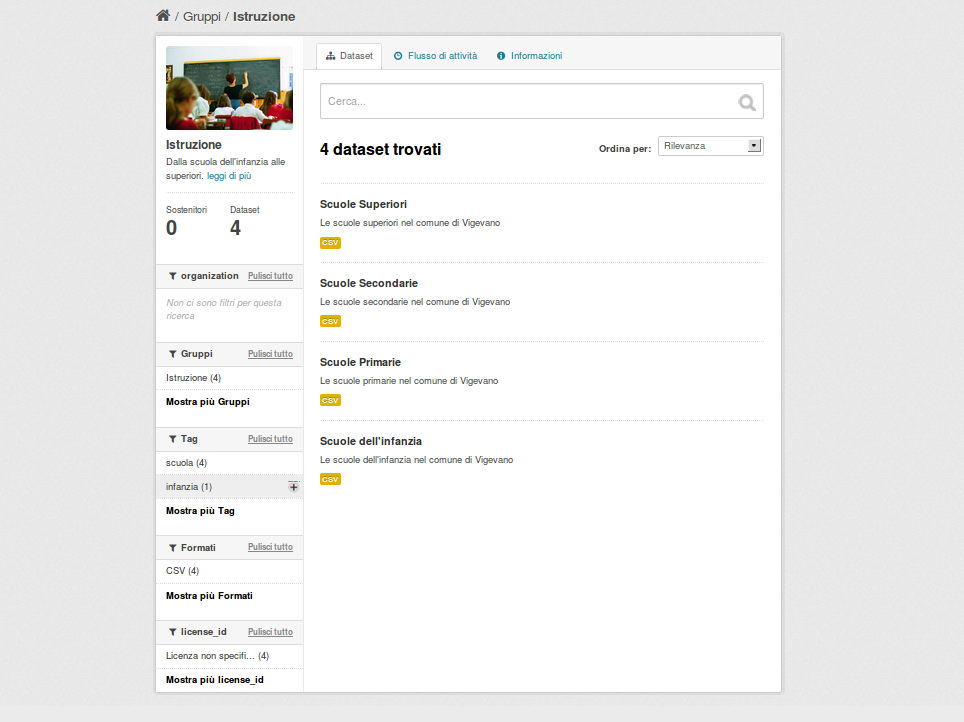
\includegraphics[scale=0.42]{img/demo-12-gruppo-dettaglio}
   \caption{Dettaglio dei dataset di un singolo gruppo}
   \label{fig:demo-12-gruppo-dettaglio}
\end{figure}


\newpage
I dati contenuti in un datset possono essere visualizzati in forma tabellare, dove � possibile ricercare una determinata informazione attraverso il campo di ricerca a destra sopra la tabella oppure attraverso i filtri (figura \ref{fig:demo-13-dataset-tabella}).

\begin{figure}[htbp]
   \centering
   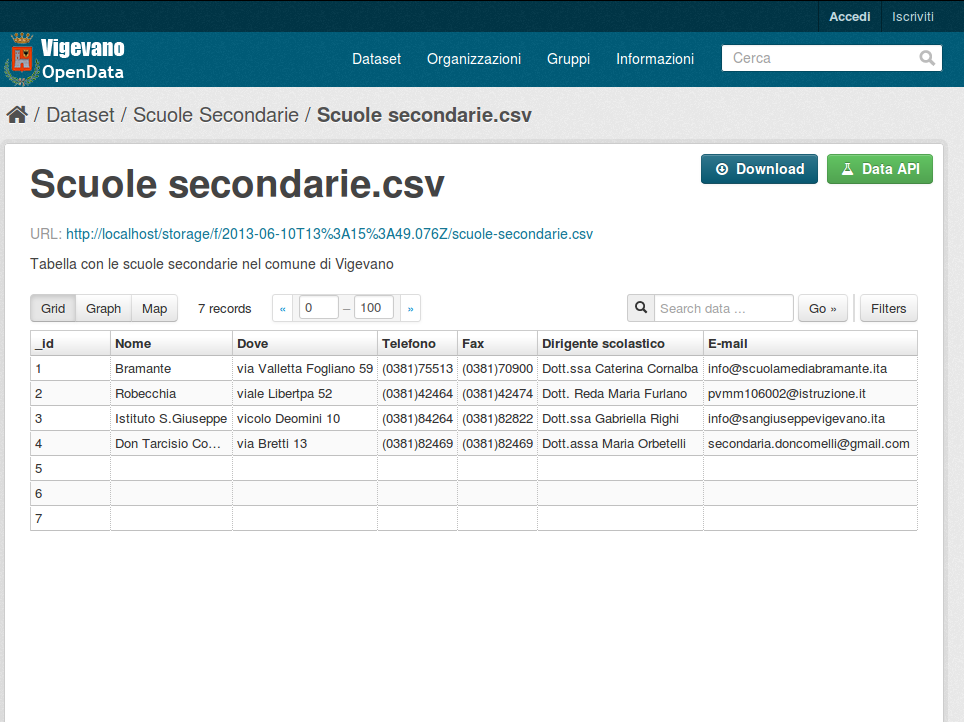
\includegraphics[scale=0.42]{img/demo-13-dataset-tabella}
   \caption{Visuale tabellare di un dataset}
   \label{fig:demo-13-dataset-tabella}
\end{figure}

\newpage
In caso esista una dipendenza tra due colonne � possibile visualizzare le informazioni attraverso dei grafici di vario tipo, ad esempio come grafico a punti o come grafico a barre (figura \ref{fig:demo-13-dataset-barre}).

\begin{figure}[htbp]
   \centering
   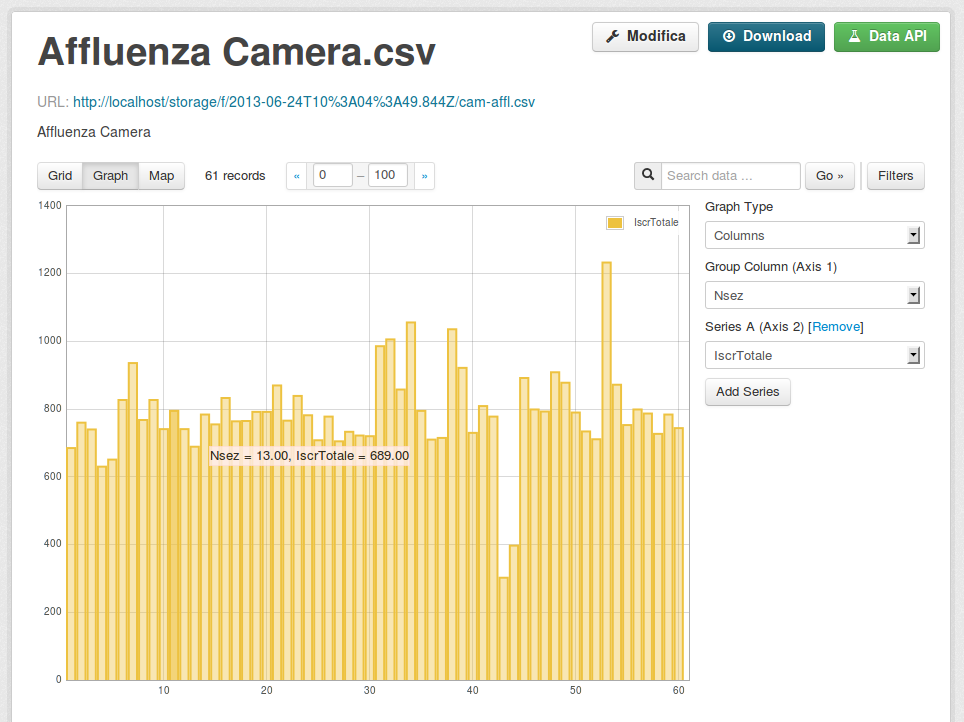
\includegraphics[scale=0.42]{img/demo-13-dataset-barre}
   \caption{Visuale a grafico di un dataset}
   \label{fig:demo-13-dataset-barre}
\end{figure}


\newpage
Infine in caso di dati geolocalizzati � possibile �mapparli� su una cartina (figura \ref{fig:demo-13-dataset-cartina}) di MapQuest. Ci� risulta veramente intuitivo per gli utenti finali.

\begin{figure}[htbp]
   \centering
   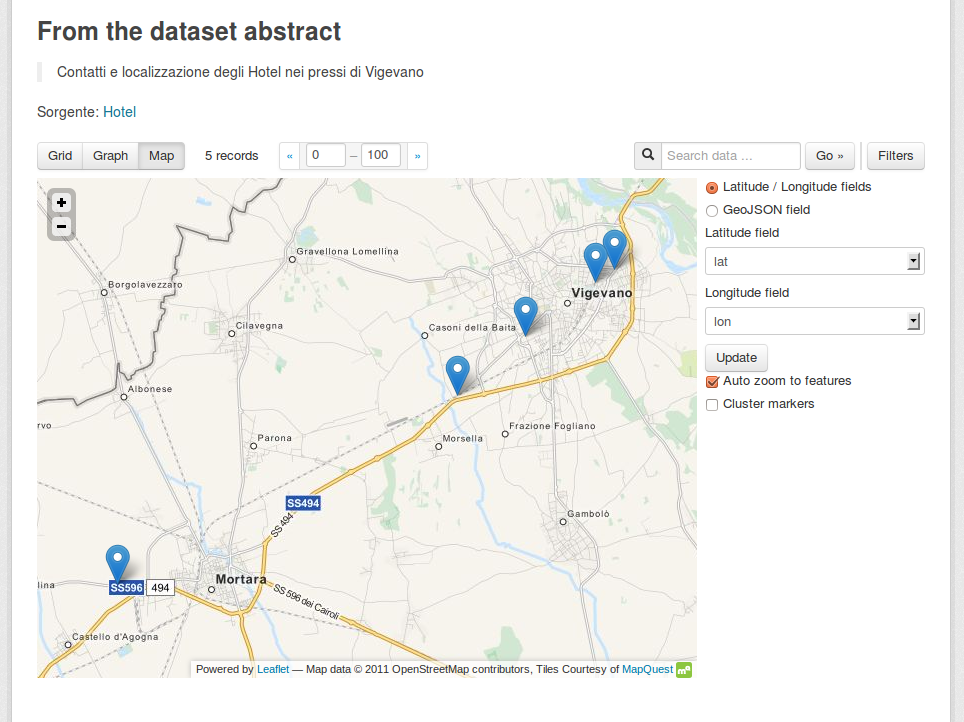
\includegraphics[scale=0.42]{img/demo-13-dataset-cartina}
   \caption{Visuale geolocalizzata di un dataset}
   \label{fig:demo-13-dataset-cartina}
\end{figure}

\newpage
Inoltre clickando su uno dei marcatori della cartina si visualizzano tutte le informazioni disponibili nel dataset relative al punto selezionato (figura \ref{fig:demo-13-dataset-cartina-dettaglio}).

\begin{figure}[htbp]
   \centering
   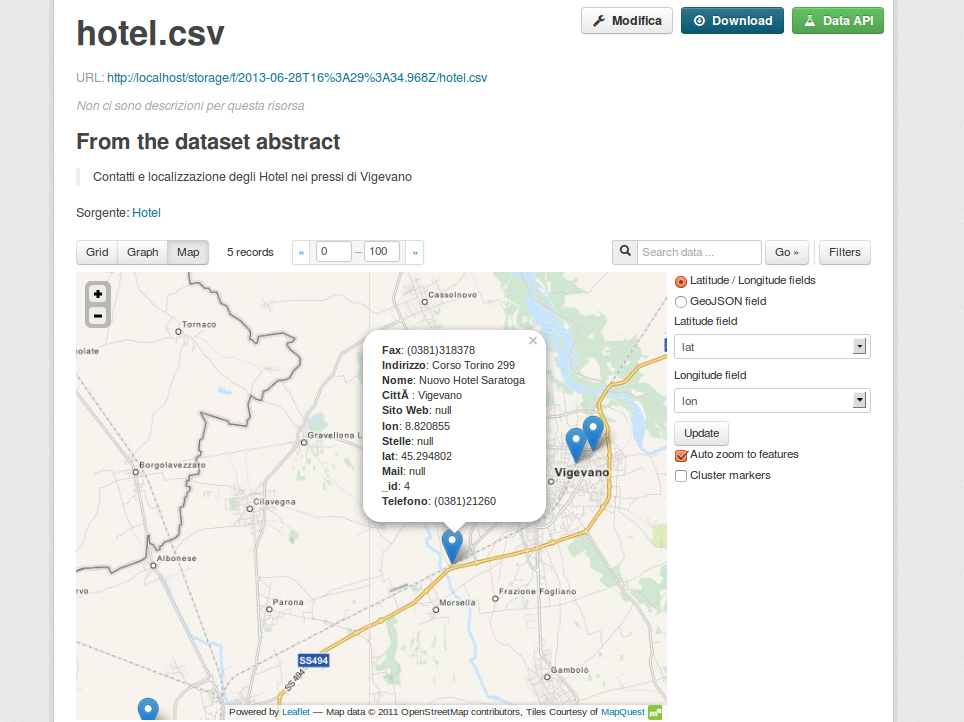
\includegraphics[scale=0.42]{img/demo-13-dataset-cartina-dettaglio}
   \caption{Dettaglio del punto selezionato sulla cartina}
   \label{fig:demo-13-dataset-cartina-dettaglio}
\end{figure}

\newpage
Man mano che nuovi dataset vengono caricati nella piattaforma il catalogo si aggiorna e si riempie delle informazioni presenti (figura \ref{fig:demo-14-datacatalog}).

\begin{figure}[htbp]
   \centering
   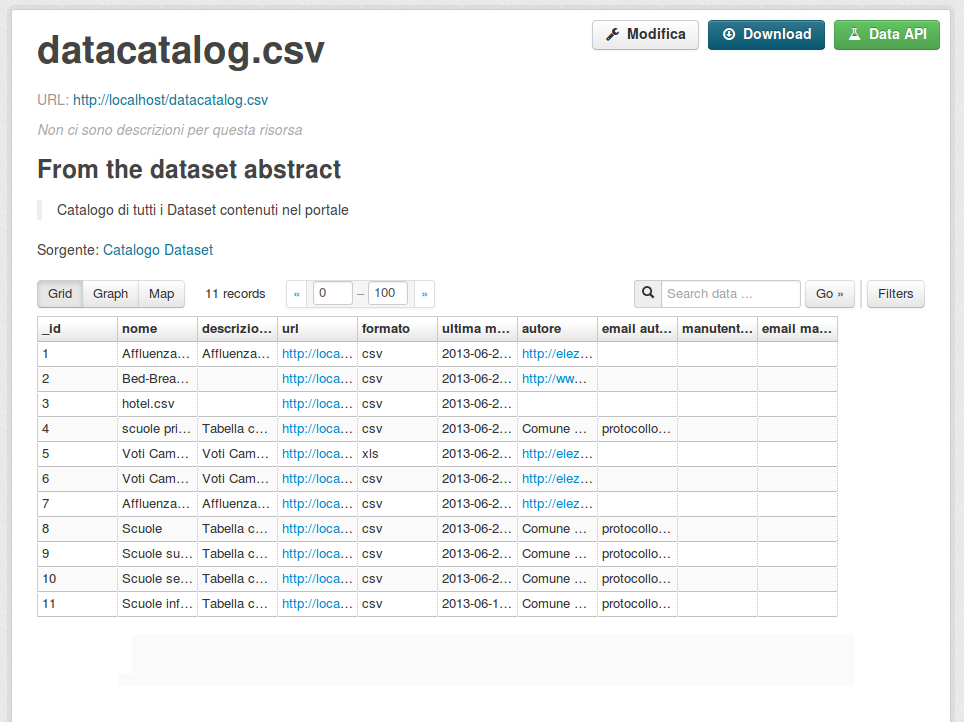
\includegraphics[scale=0.42]{img/demo-14-datacatalog}
   \caption{Catalogo dei dataset inseriti}
   \label{fig:demo-14-datacatalog}
\end{figure}
